%!TeX spellcheck = en-US

%\chapter{Evaluation Methodology for WGI and Computational Text Categorization}
\chapter{Evaluation Framework for Open-set WGI}

\label{chap:eval_methods}

%----------------------------------------------------------------------------------------

% Define some commands to keep the formatting separated from the content
\newcommand{\keyword}[1]{\textbf{#1}}
\newcommand{\tabhead}[1]{\textbf{#1}}
\newcommand{\code}[1]{\texttt{#1}}
\newcommand{\file}[1]{\texttt{\bfseries#1}}
\newcommand{\option}[1]{\texttt{\itshape#1}}

%----------------------------------------------------------------------------------------

\section{Introduction}\label{chap:eval_methods:sec:intro}

This chapter describes a framework suitable for the open-set WGI task. Particularly, using simple examples the properties of evaluation measures are demonstrated, usually adopted in closed-set classification tasks and the misleading conclusions that can be drawn in case they are also used in open-set conditions. To avoid this problem, specific evaluation measures is proposed in this thesis, specialized for the open-set WGI task.

The main difference in open-set WGI with respect to closed-set WGI is the presence of \emph{noise}. As already explained, noise can be unstructured (when the labels of web-pages not belonging to any of the known genres are not given) or structured (when the labels of web-pages not belonging to any of the known genres are given). Traditional evaluation measures do not make any distinction between known genres and the unknown class (noise). Moreover, in case of structured noise, we need a way to indicate the difficulty of the task taking into account the amount of known and unknown genres. For example, the case where we have 10 known genres and 3 unknown genres is far more difficult than the case where we have 3 known genres and 10 unknown genres. In this thesis it is propose a measure that specifically quantifies this relation and can be used to thoroughly study the performance of WGI methods.

In the rest of this chapter, first it is described the properties of well-known evaluation measures usually adopted in supervised learning tasks and discuss their suitability for open-set classification tasks. Then, the \emph{openness} measure is introduced in WGI as a means to quantify the open-space risk in the case of structured noise. Finally, the proposed evaluation framework is summarized.

\section{Evaluation Measures}
\label{chap:eval_methods:sec:measures} 

\subsection{Precision, Recall, and $F$-Score}
\label{chap:eval_methods:sec:prf_micro}

In machine learning, specifically in supervised learning, a \textit{confusion matrix} is a table that depicts the performance of an algorithm. It is a special case of a \textit{contingency table}, with two dimensions (i.e., actual and predicted). In the binary classification case, such as depicted in table \ref{chap:eval_methods:tbl:bin_confusion}, there are two classes (i.e., $A$ and $\not A$ ) and four types of results: True Positives (TP), True Negatives (TN), False Positives (FP), False Negatives (FN). TP and TN correspond to correct predictions while FP and FN are the two types of errors (they are also called Type I and Type II errors).

\begin{table}[t]
	\center
	\caption{The confusion matrix of a binary classification task}\label{chap:eval_methods:tbl:bin_confusion}
	\begin{tabular}{c c c c c}
		& & \multicolumn{2}{c}{Actual} & \\
		\cline{3-4}
		\multirow{3}{*}{\rotatebox[origin=r]{90}{Predicted}} & & \multicolumn{1}{|c}{A} & \multicolumn{1}{c|}{\neg A} &  \\
		\cline{2-4}
		& \multicolumn{1}{|c}{A} & \multicolumn{1}{|c}{\textbf{TP}} & \multicolumn{1}{c|}{FP} & \\
		& \multicolumn{1}{|c}{\neg A} & \multicolumn{1}{|c}{FN} &  \multicolumn{1}{c|}{\textbf{TN}} \\
		\cline{2-4}
		\\
	\end{tabular}
\end{table}

In order to compare the performance of binary classification algorithms, the \tetxit{Accuracy} measure can be used. This is actually the ratio of correct predictions over all available predictions (which is equivalent to the number of the samples of the whole evaluation dataset). Formally, it is defined as follows:

\begin{equation}\label{chap:eval_methods:eq:accuracy}
A = \frac {TP + TN} {TP +  TN + FP + FN}
\end{equation}

Accuracy is heavily influenced by uneven class distribution. Moreover, it gives equal weight to the two types of errors and it cannot handle cases where one of them is more important than the other. In such cases, this evaluation measure can provide misleading conclusions. 

Alternative evaluation measures that can compensate these weaknesses are \textit{Precision} and \textit{Recall}. Precision, also known as \textit{Positive Predictive Value} indicates the fraction of correct predictions for class A over all predictions while recall, also known as \textit{Sensitivity, Hit Rate and True Positive Rate} indicates the fraction of correct predictions for class A over all available instances of this class. These evaluation measures are defined as follows: 

\begin{equation}\label{chap:eval_methods:eq:precision}
	P = \frac {TP} {TP + FP}
\end{equation}

\begin{equation}\label{chap:eval_methods:eq:recall}
	R = \frac {TP} {TP + FN}
\end{equation}

There is well-known trade-off between precision and recall \parencite{Weiss2010}. Usually when one attempts to optimize one of them the other drops significantly. A popular metric that combines these two measures is called \textit{F-Score} and it is actually the harmonic mean of precision and recall which is increased when both precision and recall take high values and is reduced when at least one of them takes low values. This is defined in the following equation:

\begin{equation}\label{chap:eval_methods:eq:recall}
	F_{\beta} = (1 + \beta^{2}) \frac {P R} {\beta^{2} P + R}
\end{equation}

\noindent
where $\beta$ can be used to regulate the weighting bias towards precision or recall. Usually $F_{1}$, i.e. $\beta = 1$, is used for equally weighted precision and recall significance. If $\beta > 1$ then recall is more significant than precision and if $\beta < 1$ then precision is more important. This can be useful in specific applications where more emphasis is put on one of these two measures. Note that precision is influenced by FPs while recall is affected by FNs. For example, in email spam detection, precision is usually regarded more important than recall. It is far more important to avoid to miss-classify as spam all legal messages (FPs) than leaving some spam messages to appear in the inbox (FNs).

It is also important to note that precision and recall as well as F-score are calculated for a particular class. So far, taking into account Table \ref{chap:eval_methods:tbl:bin_confusion}, we considered A as the reference class. In general, especially when we have to deal with multi-class classification tasks, precision and recall can be calculated for each class separately. Then, we can combine these measures by taking their arithmetic mean. This provides the \textit{macro-averaged precision} and \textit{macro-averaged recall}. Let $\mathcal{C}$ be the set of classes in a multi-class classification task (e.g., in WGI this corresponds to the known genre palette) while $P_c$ and $R_c$ are the precision and recall scores of class $c \in \mathcal{C}$, respectively. Then macro-Precision (macroP) and macro-Recall (macroR) are defined as follows:

\begin{equation}\label{chap:eval_methods:eq:macro-precision}
	macroP = \frac{1}{|\mathcal{C}|} \sum_{c \in \mathcal{C}}{P_c}
\end{equation}

\begin{equation}\label{chap:eval_methods:eq:macro-recall}
	macroR = \frac{1}{|\mathcal{C}|} \sum_{c \in \mathcal{C}}{R_c}
\end{equation}

\noindent where $|\mathcal{C}|$ is the number of known classes. Accordingly, the \textit{macro F-score} can be calculated: 

\begin{equation}\label{chap:eval_methods:eq:macro-F}
	macroF = \frac{1}{|\mathcal{C}|} \sum_{c \in \mathcal{C}}{F_c}
\end{equation}

\noindent where $F_i$ is the F-score for the class $c \in \mathcal{C}$. Alternatively, one can also calculate \textit{micro-averaged precision}, \textit{micro-averaged recall}, and \textit{micro-averaged F-score}. In that case, all data samples are taken together and a single precision and recall value is calculated for all classes cumulatively. TPs correspond to correct predictions, i.e., the diagonal values in the confusion matrix.  All other cells of the confusion matrix are considered as both FPs and FNs (i.e., when a sample of class X is miss-classified to class Y this is a FN for X and a FP for Y). Thus, micro-Precision will be equal to micro-Recall and their harmonic mean  ($F_{1}$) will also be the same. Actually, micro-averaged $F_{1}$ is also equal to the accuracy measure. Consequently, micro-F is strongly dependent on the distribution of samples over the classes. On the other hand, macro-F gives equal weight to all classes.

\subsection{Open-set Variants of Evaluation Measures}

In an open-set classification task, we are given a set of known classes $\mathcal{C}$ and training samples for each $c \in \mathcal{C}$. However, in the evaluation phase the dataset may consist of both samples belonging to members of $\mathcal{C}$ and samples of classes excluded from $\mathcal{C}$. The latter (noise) can be composed of several classes. Especially in WGI, it is expected that the number of web-pages not belonging to any of the known genres would be very high. 

If one adopts the evaluation measures described in the previous section for an open-set classification task, then all samples not belonging to any $c \in \mathcal{C}$ could be considered as a single \textit{unknown} class. Then, precision, recall, and $F_{1}$ values can be obtained for this unknown class that would be considered equally important to the corresponding ones of known classes (members of $\mathcal{C}$) when calculating macro-Precision, macro-Recall, and macro-$F_{1}$. However, this implies that TPs for the unknown class is equally important with TPs for a known class. As demonstrated in \parencite{mendesjunior2016}, since there are no training samples for the unknown class and it is actually a merging of several classes, it does not make sense to consider it a single class and the evaluation measures should focus on the correct recognition of known classes.

An open-set variant of macro-Precision, macro-Recall, and macro-$F_{1}$ can be obtained by ignoring the unknown class and calculate the arithmetic mean of only the known classes \parencite{mendesjunior2016}. Equations \ref{chap:eval_methods:eq:macro-precision}, \ref{chap:eval_methods:eq:macro-recall}, and \ref{chap:eval_methods:eq:macro-F} can still be used. However, it should be underlined that in the open-set scenario the confusion matrix has $|\mathcal{C}|+1$ rows/columns. This means that one class (the unknown class) is ignored when calculating the macro-averaged scores. On the other hand, the samples of the unknown class that are miss-classified to the known classes (false known) and the samples of the known classes miss-classified as unknown (false unknowns) still affect the precision and recall of known classes, respectively. 

Similar to open-set macro-averaged scores, open-set micro-averaged precision, recall, and $F_{1}$ can be obtained. Note that in this case, micro-precision is not necessarily equal to micro-recall since the former is affected by the presence of false known and the latter is affected by false unknowns. Again, the TPs of the unknown class are ignored. 

We provide an illustrating example that demonstrates the difference between traditional evaluation measures and their open-set variance. Table \ref{chap:eval_methods:tbl:multi_confusion} shows an example of a confusion matrix for an open-set classification task with four known classes ($\mathcal{C}=\{A,B,C,D\}$). In WGI, this could correspond to a genre palette of four known genres (e.g. blogs, e-shop, home pages, discussion) for which training samples are available. As can be seen, there are 20 evaluation samples for each known class and 200 samples of the unknown class ($\emptyset$). This is realistic since in practice noise is expected to outnumber any given known genre. Correct predictions (TPs) are in boldface. Table \ref{chap:eval_methods:tbl:prec_rec_f1_example} shows the precision, recall, and $F_{1}$ scores for all, both known and unknown, classes. In addition, Table \ref{chap:eval_methods:tbl:closed_vs_open} demonstrates the traditional macro-averaged and micro-averaged precision, recall, and $F_{1}$ as well as their corresponding open-set variant. Note that in the former the set $\mathcal{C} \cup \emptyset$ is used while in the latter is based on $\mathcal{C}$. 

The table \ref{chap:eval_methods:tbl:bin_confusion} has $140$ total samples which is equal either the the row-sums or the column-sums are summed up. In the case of open-set classification some of the samples are remaining as non-classification or as \textit{unknown} where there is no class trained for them. 

In table \ref{chap:eval_methods:tbl:multi_confusion} there are still 140 sample distributed in a seven (7) classes and also with 42 of them remaining as unclassified. Given these cases, the respective per class, macro and micro recall for this confusion matrix are calculated and shown in table \ref{chap:eval_methods:tbl:macro_vs_micro}.

\begin{table}[t]
	\center
	\caption{Confusion metric of binary classification}\label{chap:eval_methods:tbl:multi_confusion}
	\begin{tabular}{c c c c c c c c}
		& & \multicolumn{6}{c}{Actual} & \\
		\cline{3-7}
		\multirow{7}{*}{\rotatebox[origin=c]{90}{Predicted}} & & \multicolumn{1}{|c}{A} & \multicolumn{1}{c}{B} & \multicolumn{1}{c}{C} & \multicolumn{1}{c}{D} & \multicolumn{1}{c|}{\emptyset} & \\
		\cline{2-7}
		& \multicolumn{1}{|c}{A} & \multicolumn{1}{|c}{\textbf{13}} & \multicolumn{1}{c}{2} & \multicolumn{1}{c}{0} & \multicolumn{1}{c}{0} & \multicolumn{1}{c|}{0} & 15 \\
		& \multicolumn{1}{|c}{B} & \multicolumn{1}{|c}{1} & \multicolumn{1}{c}{\textbf{10}} & \multicolumn{1}{c}{0} & \multicolumn{1}{c}{0} & \multicolumn{1}{c|}{10} & 21 \\
		& \multicolumn{1}{|c}{C} & \multicolumn{1}{|c}{0} & \multicolumn{1}{c}{0} & \multicolumn{1}{c}{\textbf{8}} & \multicolumn{1}{c}{0} & \multicolumn{1}{c|}{0} & 8 \\
		& \multicolumn{1}{|c}{D} & \multicolumn{1}{|c}{0} & \multicolumn{1}{c}{0} & \multicolumn{1}{c}{2} & \multicolumn{1}{c}{\textbf{20}} & \multicolumn{1}{c|}{10} & 32 \\
		& \multicolumn{1}{|c}{\emptyset} & \multicolumn{1}{|c}{\textit{6}} & \multicolumn{1}{c}{\textit{8}} & \multicolumn{1}{c}{\textit{10}} & \multicolumn{1}{c}{\textit{0}} & \multicolumn{1}{c|}{\textbf{180}} & {204} \\
		\cline{2-7}
		% & & 0 & 14 & 12 & 11 & 12 & 20 & 13 & 16 & \textbf{70}\\
		% \cline{3-11}
		& & \textit{20} & \textit{20} & \textit{20} & \textit{20} & \textit{200} & \textbf{231}\\
	\end{tabular}
\end{table}


\begin{table}[H][t]
	\center
	\caption{Macro and Micro calculation for the Confusion matrix (Table \ref{chap:eval_methods:tbl:multi_confusion}) of multi-class classification}\label{chap:eval_methods:tbl:macro_vs_micro}
	\begin{tabular}{l l l}
		\cline{2-3}
		& \multicolumn{1}{|c}{Precision} & \multicolumn{1}{c|}{Recall}\\
		\cline{1-3}
		\multicolumn{1}{|c}{A} & \multicolumn{1}{|c}{0.866} & \multicolumn{1}{c|}{0.650}\\
		\multicolumn{1}{|c}{B} & \multicolumn{1}{|c}{0.476} & \multicolumn{1}{c|}{0.500}\\
		\multicolumn{1}{|c}{C} & \multicolumn{1}{|c}{1.000} & \multicolumn{1}{c|}{0.400}\\
		\multicolumn{1}{|c}{D} & \multicolumn{1}{|c}{0.625} & \multicolumn{1}{c|}{1.000}\\
		\multicolumn{1}{|c}{\emptyset} & \multicolumn{1}{|c}{0.882} & \multicolumn{1}{c|}{0.900}\\
		\cline{1-3}
		\multicolumn{1}{|c}{Macro ($\mathcal{C}$)} & \multicolumn{1}{|c}{0.741} & \multicolumn{1}{c|}{0.638}\\
		\multicolumn{1}{|c}{Macro ($\mathcal{C} \cup \emptyset$)} & \multicolumn{1}{|c}{0.770} & \multicolumn{1}{c|}{0.690}\\
		\multicolumn{1}{|c}{Micro ($\mathcal{C}$)} & \multicolumn{1}{|c}{0.632} & \multicolumn{1}{c|}{0.600}\\
		\multicolumn{1}{|c}{Micro ($\mathcal{C} \cup \emptyset$)} & \multicolumn{1}{|c}{0.825} & \multicolumn{1}{c|}{0.825}\\
		\cline{1-3}
	\end{tabular}
\end{table}


Clearly the is a significant difference in the macro-P compare to the micro-P and for this case, micro and macro recalls are have both $0.500$ score. It should be noted that due to the 42 samples of the 140 that haven't been classified at all there is bias over precision score when its micro score is calculated. Moreover, there is problem in calculation of the recall based in the equation form \ref{chap:eval_methods:eq:recall} because in the closed set classification the denominator is equal to the total number pf samples that we know they are under the distribution of the class we are evaluating for. 

The recall calculation issue is cased because of the open-set framework and the sample are renaming out of the classification processing because of the rejection criterion of an open-set algorithm. In order to calculate the recall we are following the theoretical definition of the this score which is formally expressed in equation \ref{chap:eval_methods:eq:recall_theory}.

\begin{equation}\label{chap:eval_methods:eq:recall_theory}
	R = \frac {\text{The sum of correctly classified samples}} {\text{The total number of distribution's testing samples}}
\end{equation}

Thus in the case of \textit{micro-R} is the denominator is equal to the total number of all samples of the data-set. In the \textit{macro-R} case, is the number of the class-samples for every class separately and then the average score recall score of all classes.

In the table \ref{chap:eval_methods:tbl:multi_confusion} the micro recall show that only the $50\%$ of the total samples have been correctly classified and the $98/140 = 70\%$ of the total samples have been classified while the rest has been remained as \textit{unknown}. The macro recall is also $0.500$ based on the separated evaluation for every different class.

However, the precision is much more accurate in the case of macro compare to the micro because the micro precision is bias for the algorithms positive performance since the rejected samples (characterized as unknown) are not calculate in the precision performance or their are not causing any kind of penalty to the precision score. In addition the proper calculation of recall (micro and macro) as explained above will not differ in the extend of regulating the F-score.

The macro scores are then less biased for the the open-set framework evaluation. Moreover, in the highly imbalanced corpora also the macro scoring is reported to be more realistic and less biased. Due to the above reasoning the macro-P, macro-R, and Macro-F1 will mainly be the evaluation measure is used in this thesis.

In the next chapter the Precision Recall Curves will be presented where it is more vivid the effect of the micro and macro measurement. That is there it is clear the bias over the precision in the algorithm's performance because of the open-set algorithm criterion.


\subsection{Precision-Recall Curves}\label{chap:eval_methods:sec:roc_prc}

So far, the evaluation measures consider classification algorithms that provide crisp predictions (i.e., \textit{hard classifiers}). The discussed evaluation measures are only available to show particular aspects of the performance of classifiers. To obtain a deeper look we need richer evaluation methods that can depict the performance of classifiers in a variety of conditions. One such method is the \textit{Precision-Recall Curves (PRC)}, a standard method for evaluating information retrieval systems and ranking systems. They can only be applied to \textit{soft classifiers} that are able to explicitly estimate class conditional probabilities. Fortunately, the vast majority of hard classifiers can be adopted to also provide some form of score that can be regarded as class conditional probability.

The calculation of a PRC requires the ranking of estimated probabilities in descending order. In each step, the next prediction is considered and a new precision and recall point is calculated. Both macro-PRC and micro-PRC can be calculated.

In order to facilitate the comparison of PRCs corresponding to the performance of different systems on the same evaluation dataset, the 11-recall level normalization is typically used. The initial points of PRC are reduced to 11 that correspond to standard recall levels $[0,0.1,...,1.0]$. For example, in case Recall$=0.1$, we measure precision when 10\% of the samples have been seen. Precision values are interpolated based on the following formula:

\begin{equation}\label{chap:eval_methods:eq:11recall_level}
	P(r_j)=max_{r_j \leqslant r \leqslant r_{j+1}}(P(r))
\end{equation}

\noindent
where $P(r_j)$ is the precision at $r_j$ standard recall level ($r_j=\{0,0.1,0.2,...,1.0\}$).

\begin{table}[t]
	\center
	\caption{Macro and Micro calculation for the Confusion matrix (Table \ref{chap:eval_methods:tbl:multi_confusion}) of binary classification}\label{chap:eval_methods:tbl:prc}
	\begin{tabular}{|c|c|c|c|}
		\cline{1-4}
		Certainty & Predicted & Expected & Correct\\
		\cline{1-4}
		0.99 & 1 & 1 & 1 \\
		0.99 & 2 & 2 & 1 \\
		0.99 & 4 & 4 & 1 \\
		... & ... & ... & ... \\
		0.79 & 2 & 6 & 0 \\
		0.79 & 4 & 4 & 1 \\
		0.69 & 7 & 6 & 0 \\
		0.69 & 4 & 4 & 1 \\
		... & ... & ... & ... \\
		0.64 & \emptyset & 6 & 0 \\
		0.60 & 2 & 2 & 1 \\
		... & ... & ... & ... \\
		0.60 & \emptyset & 4 & 0 \\
		\cline{1-4}
	\end{tabular}
\end{table}

In table \ref{chap:eval_methods:tbl:prc} it is shown an sequence of calculation for the corpus formed the final confusion matrix of table \ref{chap:eval_methods:tbl:multi_confusion}. In this case, an open-set algorithm returned the predictions together with its certainty scores. 

\begin{figure}[t]
	\begin{center}
    	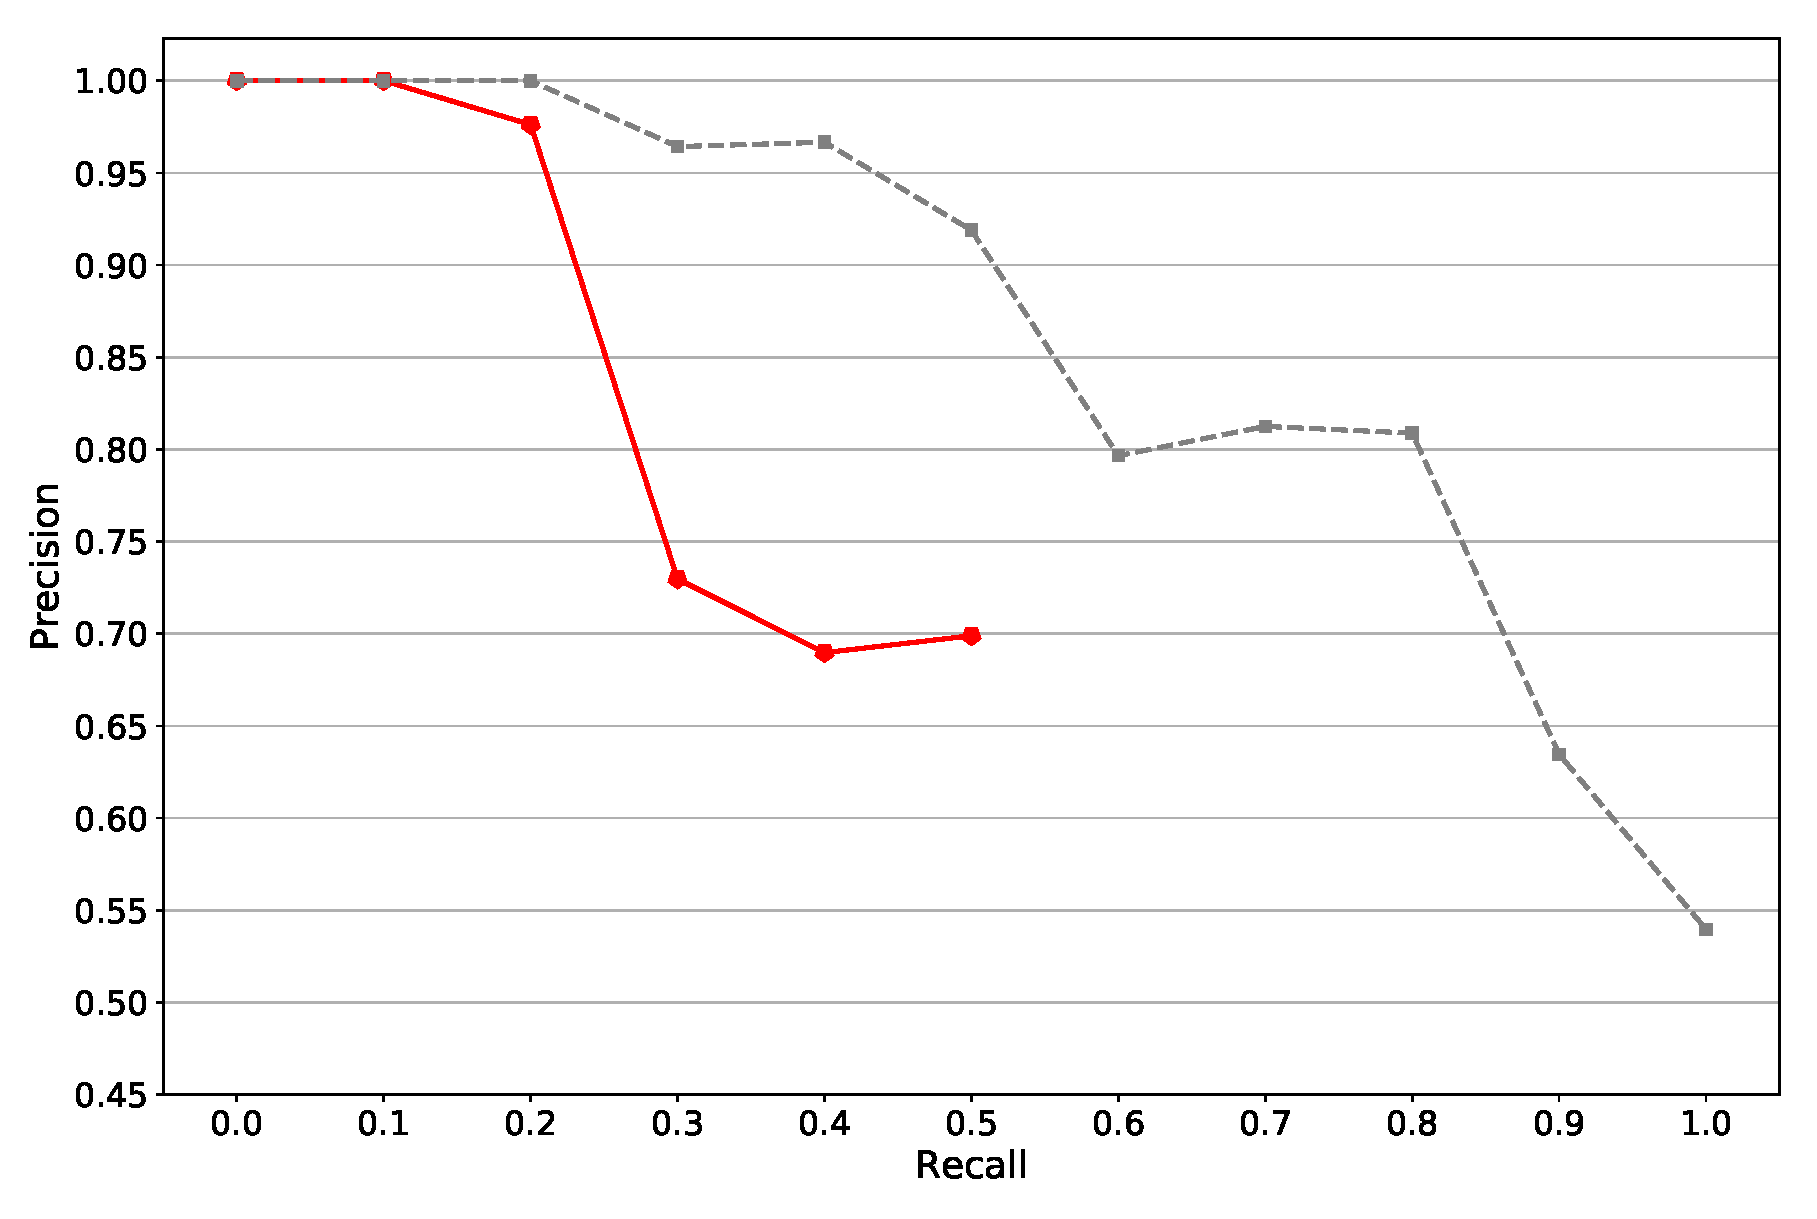
\includegraphics[scale=0.45]{Figures/pr_macro_micro_example.eps}
		\caption{Open-set Macro (Red line) and Micro (grey line) Precision Recall Curves of confusion matrix in table \ref{chap:eval_methods:tbl:multi_confusion}}
		\label{chap:eval_methods:fig:prc_macro}
	\end{center}
\end{figure}

The two curves yielding from this calculations, micro and macro PRC are shown in figure \ref{chap:eval_methods:fig:prc_macro}. Clearly, the micro-PRC is misleading compare to the macro-PRC and the results of table \ref{chap:eval_methods:tbl:macro_vs_micro}. 

The macro-P is measures (in table \ref{chap:eval_methods:tbl:macro_vs_micro}) are leading to the conclusion of a low performance algorithm, especially for the recall score. On the contrary the micro-P is leading to the conclusion of a high performance algorithm, which we know that it is not true, form the confusion matrix of \ref{chap:eval_methods:tbl:multi_confusion}.

To compensate the potentially unbalanced distribution of web pages over the genres, the macro-averaged precision and recall measures is used. In more detail, in this thesis a modified version of precision and recall is used, for open-set classification tasks proposed by \parencite{mendesjunior2016}. This modification calculates precision and recall only for the known classes (available in the training phase) while the unknown samples (belonging to classes not available during training) affect false positives and false negatives.

The problem of the misleading micro-PRC is cased by the presence of the outages, depicted in the first row, in the confusion matrix \ref{chap:eval_methods:tbl:multi_confusion}. Particularly, as shown in table \ref{chap:eval_methods:tbl:prc} and the rows 10 and 13, the micro-PRC calculation is considering the rejected incorrect predicted and it is including them in the prediction. Thus these predictions are not calculated in the precision equation \ref{chap:eval_methods:eq:precision}. These predictions are just decreasing the micro-R. Consequently, the curve is overestimating the performance of the algorithm.

On the contrary the macro-PRC is closer to the macro prediction and recall. Particularly it is show that the curve stops near the $0.5$ values which is equal to the macro-R. Moreover, macro-precision is high yet drops significantly due to the $0.60$. The PRC is giving the same evaluation performance with the table's \ref{chap:eval_methods:tbl:macro_vs_micro} scores per class and macro-scores. That is, the algorithm is having really good performance for some classes and really bad for some other.

However, due to the certainty ranking we can see more insight related to the algorithms performance. Particularly, we can see some irregular drops in the micro-PRC. Also the slope of the macor-PRC first recall level to the second is very small and then drops from the near perfect predictions to the $0.87$ precision etc. Also, the curve it stops at $0.5$ recall level.

These, Micro-PRC (and some time in Macro-PRC) 'irregular' properties are only meet at the open-set algorithms because of the rejection factor. In table \ref{chap:eval_methods:tbl:prc} the algorithms of the precision in rows 10 and 13, seems to have $0.60$ certainty factor which is almost as high as its correct predictions. These predictions are casing high fluctuations in the PRC which are regularized because the 11-recall level average normalization is applied on top. 


\section{Area Under the Curve (AUC)}\label{chap:eval_methods:sec:closed_set_classification} 

In table \ref{chap:eval_methods:tbl:AUC_F1} the Micro and Macro \textit{Area Under the Curve (AUC)} and F1 are presented. The AUC is a common values is used when several PRC's needs to be compared. As an example, to find parameter settings that obtain optimal evaluation performances for the open-set algorithms, the AUC for the PRC's of figure \ref{chap:eval_methods:fig:prc_macro} can be calculated. 


\begin{table}[t]
	\center
	\caption{Macro and Micro calculation for AUC and F1 of the Confusion matrix (Table \ref{chap:eval_methods:tbl:multi_confusion})}\label{chap:eval_methods:tbl:AUC_F1}
	\begin{tabular}{c|c|c|}
		\cline{2-3}
		& AUC & F1 \\
		\hline
		\multicolumn{1}{|c|}{Macro} & 0.448 & 0.570 \\
		\multicolumn{1}{|c|}{Micro} & 0.866 & 0.588 \\	
		\hline
	\end{tabular}
\end{table}

It is very important to note that the Micro-AUC is highly misleading, as expected from the PRC diagram \ref{chap:eval_methods:fig:prc_macro}. On the contrary the F1 is not so different, although, as explained, is overestimating the performance o the algorithm by overestimating the precision score. 

The effect of a this potential misleading choice, selecting the \textit{micro-scores} instead of the \textit{macro-scores}, is a bad choice of the  hyper-parameters required for the proper tuning of the classification algorithm. In the experiments (chapter \ref{chap:noise}) of this thesis, it will pointed out whenever this danger is occurring.

\section{The Openness Test}\label{chap:eval_methods:sec:openness}

The open-set evaluation measures defined in this chapter can be used in both unstructured and structured noise. However, in the latter case, we need a more detailed analysis of the performance to indicate the ability of the open-set classifier to handle low/high number of training/unknown classes. It is especially important to study the relation of the number of training classes with respect to the number of unknown classes. 

In \parencite{scheirer2013toward}, the \textit{openness measure} is introduced to directly measure this relation. The openness measure indicates the difficulty of an open-set classification task by taking into account the number of \textit{training classes} (i.e. the known classes used in the training phase) and the number of \textit{testing classes} (i.e., both known and unknown classes used in the testing phase) \parentcite{mendesjunior2016}:

\begin{equation}\label{chap:eval_methods:eq:openness}
	openness=1-\sqrt{\frac{ | Training Classes | }{ |Testing Classes | }}
\end{equation}

When openness is $0.0$, it is essentially a closed-set task, that is the training and testing classes are exactly the same. This actually means that there is no noise. At the other extreme, when openness reaches $1.0$ this means that the known classes are far less than the unknown classes or that the amount of noise is especially high and heterogeneous. Therefore, by varying the openness level we can study the performance of WGI models in different conditions.

Note that the openness measure can only be applied to datasets where all available samples have been labeled with class information. In the case of WGI, we have to know the genre labels of the pages that form the noise (i.e. structured noise). This information is only used to quantify the homogeneity of the noise.

The study of open-set classifiers can be significantly extended by measuring their performance (e.g., $macro F_{1}$) for varying values of the openness score. Given that $\mathcal{U}$ is the set of unknown classes (structured noise) it is possible to vary the training classes from 1 to $|\mathcal{c}|$ while the testing classes can vary from $|\mathcal{C}|$ to $|\mathcal{C}|+|\mathcal{U}|$. 

\begin{figure}[t]
	\begin{center}
    	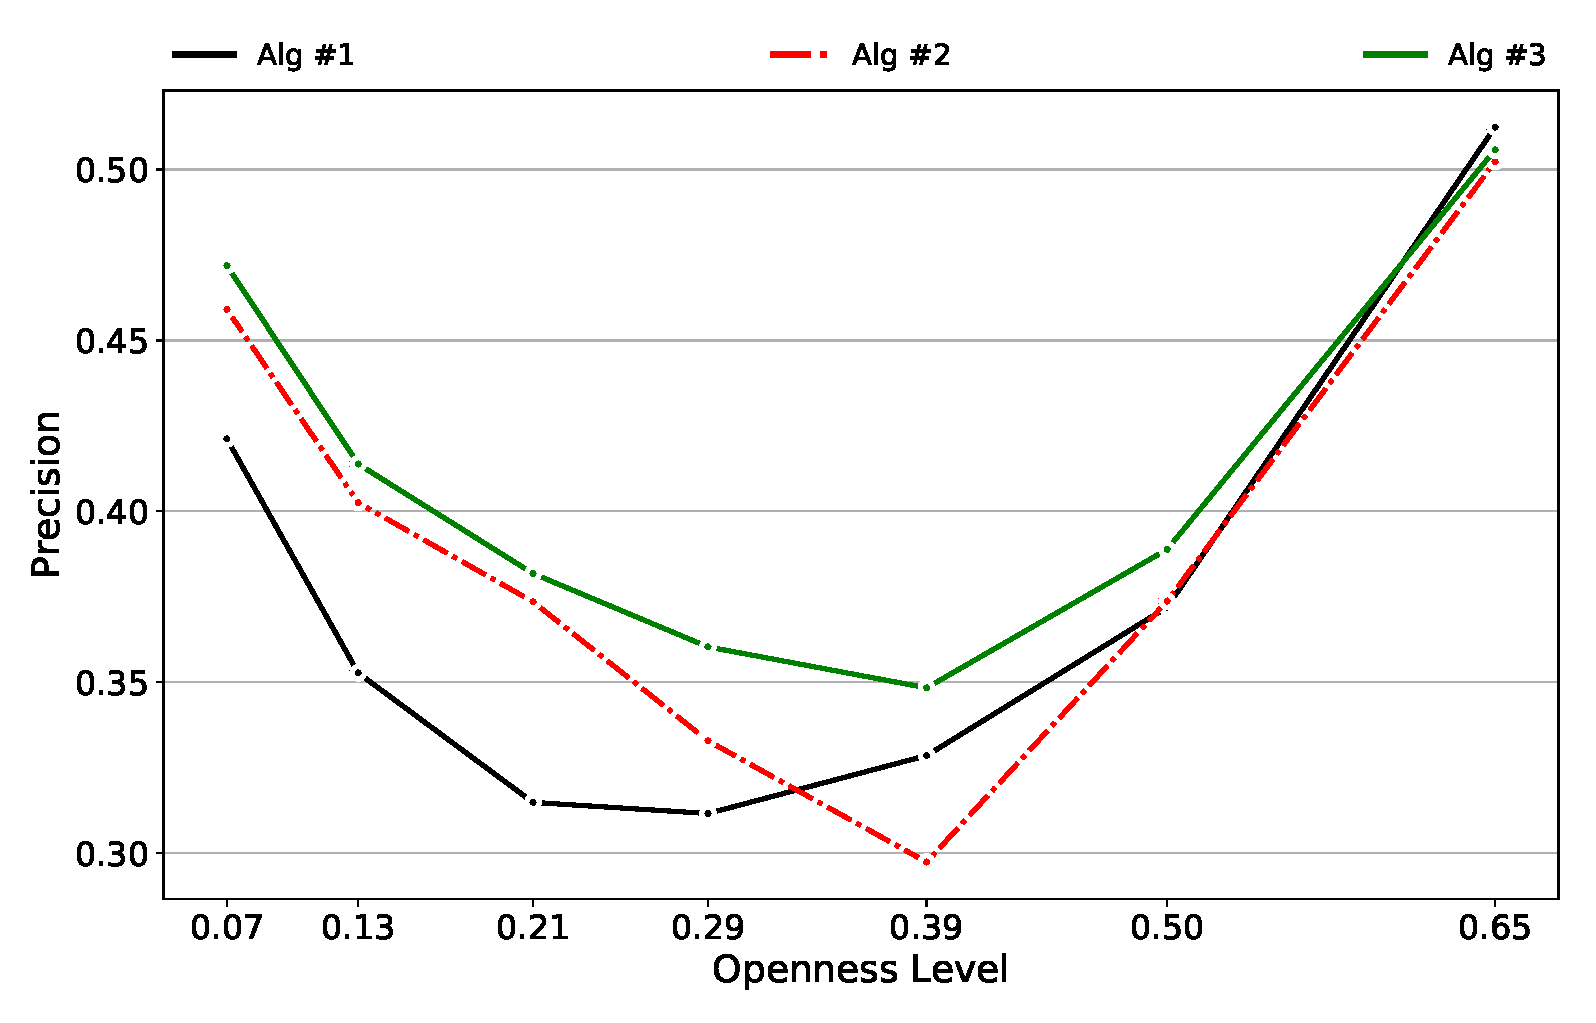
\includegraphics[scale=0.50]{Figures/openness_example.eps}
		\caption{An example of using the openness test. The smallest openness level corresponds to 6 training classes and 7 testing classes. The maximum openness level refers to 1 training class and 7 testing classes. At the 1.7 the the openness score is maximized for this open-set problem.}
		\label{chap:eval_methods:fig:openness}
	\end{center}
\end{figure}

In figure \ref{chap:eval_methods:fig:openness} the precision scores on different openness levels, are presented for evaluating three arbitrary open-set algorithms, on the corpus which it is forming the confusion matrix \ref{chap:eval_methods:tbl:multi_confusion}. Note, that the begging and the end of the curve are pointing at about the same level of precision. In particular, at the maximized openness level the performance of these algorithms is even higher than the one at the lowest openness level. However, at the begging the problem is still remaining a multi-class problem where 6 known classed have been given to the algorithms for training and 7 for testing where only 1 is unknown. However, at the highest openness level the problem is becoming a binary problem as in 1-vs-Rest. That is, the algorithms are trained at 1 class and tested at 7 classes with 6 of them as unknown. Given, that these algorithms are all variations based on SVM algorithms the results are short of expected. However, this is not always the case as it will be shown in chapter \ref{chap:noise}.


\subsection{Domain Transfer Measure}\label{chap:eval_methods:sec:domain_transfer_measure}

\textit{Domain Transfer Evaluation (DTE)} is a practical methodology for evaluating the classification performance of an text-mining algorithm. The goal of this evaluation methodology is to measure the generalization of the algorithm's induced model when the training corpus is rather small. Thus, with the domain transfer evaluation the algorithm's performance is tested in an unknown domain, for the same text-mining task. 

Particularly for the WGI, with this measure we can evaluate an algorithm that has been trained to identify \textit{News} or \textit{Wiki} genres. Then by testing it on \textit{Blog}, we could evaluate the model in such a case when very small corpus is available for training. Also, DTE can be applied for evaluating the model's behavior upon changes of the type of \textit{features} have been selected, e.g. BOW, POS, Term N-grams etc. 

The performance it can be measured using Accuracy, F1-statistic, Precision-Recall Curve, Receiver Operating Characteristic (ROC) Curve etc, and then compare the two measures pairwise for every domain combination (e.g. $\{News, Sports\}$, etc).

The measure proposed from \parencite{finn2006learning} where equation \ref{chap:eval_methods:eq:office_doc_ensemble} is its generalized form. Originally, this measure was designed for \textit{Accuracy} in mind. However, it can be used for any score such as F1. In order to fit in the open-set framework.

\begin{equation} \label{chap:eval_methods:eq:office_doc_ensemble}
	T^{C,F} = \frac{1}{N(N-1)} \sum_{A=1}^{N} \sum_{B, \forall B \neq A}^{N} \left(  \frac{M^{C,F}_{A,B}}{M^{C,F}_{A,A}} \right)
\end{equation}

\noindent	
where T is the \textit{Transfer Measure Score}, M is the measure of choice (Accuracy, F1, Precision, Recall, etc), F is the \textit{Feature Set}, and C is the \textit{Genre Class}. 


\section{Conclusions}

In this chapter we discussed evaluation measures that can be used for open-set classifiers. We demonstrated that traditional precision, recall, and $F_{1}$ measures are misleading since they take into account the unknown class (noise) as a single regular class. However, since this is an heterogeneous class should not be treated equally with the training classes. For that reason, modifications of these evaluation measures, the open-set precision, recall, and $F_{1}$ are more appropriate since the TPs of the unknown class are ignored. For open-set WGI, where the noise is usually not only highly heterogeneous but also significantly outnumbers the known classes, the use of the open-set variants of the measures is considered very important.

Another main direction is the use of graphical evaluation methods that better depict the performance of open-set classifiers in various conditions. We suggest the use of two such measures, the precision-recall curves on 11-standard recall levels and the openness test. The former provides a detailed view of the performance of an open-set WGI system that suits any given application (e.g., in ranking applications, precision at low recall levels is of paramount important). The latter provides a direct control of the difficulty of the task in structured noise and can demonstrate the performance of the classifiers in varying conditions, from cases very similar to the closed-set scenario where noise is homogeneous to ones where the structured noise is highly heterogeneous.

In the next chapters we will adopt the evaluation principles described here to evaluate the open-set WGI algorithms introduced in this thesis.